%%%%%%%%%%%%%%%%%%%%%%%%%%%%%%%%%%%%%%%%%
% Short Sectioned Assignment LaTeX Template Version 1.0 (5/5/12)
% This template has been downloaded from: http://www.LaTeXTemplates.com
% Original author:  Frits Wenneker (http://www.howtotex.com)
% License: CC BY-NC-SA 3.0 (http://creativecommons.org/licenses/by-nc-sa/3.0/)
%%%%%%%%%%%%%%%%%%%%%%%%%%%%%%%%%%%%%%%%%

%----------------------------------------------------------------------------------------
%	PACKAGES AND OTHER DOCUMENT CONFIGURATIONS
%----------------------------------------------------------------------------------------

\documentclass[paper=a4, fontsize=11pt]{scrartcl} % A4 paper and 11pt font size
% ---- Entrada y salida de texto -----

\usepackage[T1]{fontenc} % Use 8-bit encoding that has 256 glyphs
\usepackage[utf8]{inputenc}
\usepackage{fourier} % Use the Adobe Utopia font for the document - comment this line to return to the LaTeX default
% ---- Idioma --------

\usepackage[spanish, es-tabla]{babel} % Selecciona el español para palabras introducidas automáticamente, p.ej. "septiembre" en la fecha y especifica que se use la palabra Tabla en vez de Cuadro

% ---- Code insertion ----
\usepackage{minted}
\usepackage{tcolorbox}
\BeforeBeginEnvironment{minted}{\begin{tcolorbox}}%
	\AfterEndEnvironment{minted}{\end{tcolorbox}}%
\setminted{
fontsize=\small,
breaklines,
breaksymbolleft=
}
% ---- Otros paquetes ----
\usepackage{dirtree}

\usepackage{url} % ,href} %para incluir URLs e hipervínculos dentro del texto (aunque hay que instalar href)
\usepackage{hyperref} % ,href} %para incluir URLs e hipervínculos dentro del texto (aunque hay que instalar href)
\hypersetup{
	colorlinks=true,
	linkcolor=blue,
	filecolor=magenta,      
	urlcolor=blue,
}

\usepackage{xcolor}
\definecolor{light-gray}{gray}{0.95}
\definecolor{alizarin}{rgb}{0.82, 0.1, 0.26}
\definecolor{nyellow}{rgb}{0.91, 0.656, 0.0}
%\definecolor{indigo}{rgb}{0.29, 0.0, 0.51}
%	\textcolor{red}{p}
%	\textcolor{orange}{r}
%	\textcolor{yellow}{a}
%	\textcolor{green}{c}
%	\textcolor{blue}{t}
%	\textcolor{indigo}{i}
%	\textcolor{violet}{c}
%	\textcolor{red}{a}
%	\textcolor{orange}{s}
%	\textcolor{yellow}{,}
%	\textcolor{green}{I}
%	\textcolor{blue}{S}
%	\textcolor{indigo}{E}

\usepackage{amsmath,amsfonts,amsthm} % Math packages
%\usepackage{graphics,graphicx, floatrow} %para incluir imágenes y notas en las imágenes
\usepackage{graphics,graphicx, float} %para incluir imágenes y colocarlas
\usepackage[export]{adjustbox}
\graphicspath{{imagenes/}}

% Para hacer tablas comlejas
%\usepackage{multirow}
%\usepackage{threeparttable}

%\usepackage{sectsty} % Allows customizing section commands
%\allsectionsfont{\centering \normalfont\scshape} % Make all sections centered, the default font and small caps

%Remove warnings
\usepackage{silence}
\WarningFilter{scrartcl}{Usage of package `fancyhdr'}

\usepackage{fancyhdr} % Custom headers and footers
\pagestyle{fancyplain} % Makes all pages in the document conform to the custom headers and footers
\fancyhead{} % No page header - if you want one, create it in the same way as the footers below
\fancyfoot[L]{} % Empty left footer
\fancyfoot[C]{} % Empty center footer
\fancyfoot[R]{\thepage} % Page numbering for right footer
\renewcommand{\headrulewidth}{0pt} % Remove header underlines
\renewcommand{\footrulewidth}{0pt} % Remove footer underlines
\setlength{\headheight}{13.6pt} % Customize the height of the header

\numberwithin{equation}{section} % Number equations within sections (i.e. 1.1, 1.2, 2.1, 2.2 instead of 1, 2, 3, 4)
\numberwithin{figure}{section} % Number figures within sections (i.e. 1.1, 1.2, 2.1, 2.2 instead of 1, 2, 3, 4)
\numberwithin{table}{section} % Number tables within sections (i.e. 1.1, 1.2, 2.1, 2.2 instead of 1, 2, 3, 4)

\setlength\parindent{0pt} % Removes all indentation from paragraphs - comment this line for an assignment with lots of text

\newcommand{\horrule}[1]{\rule{\linewidth}{#1}} % Create horizontal rule command with 1 argument of height

%----------------------------------------------------------------------------------------
%	TÍTULO Y DATOS DEL ALUMNO
%----------------------------------------------------------------------------------------

\title{	
\normalfont \normalsize 
\textsc{\textbf{Ingeniería de Servidores (2022-2023)} \\ Grado en Ingeniería Informática \\ Universidad de Granada} \\ [25pt] % Your university, school and/or department name(s)
\horrule{0.5pt} \\[0.4cm] % Thin top horizontal rule
\huge Memoria Práctica 3 \\ % The assignment title
\horrule{2pt} \\[0.5cm] % Thick bottom horizontal rule
}

\author{Yeray López Ramírez} % Nombre y apellidos

\date{\normalsize\today} % Incluye la fecha actual

%----------------------------------------------------------------------------------------
% DOCUMENTO
%----------------------------------------------------------------------------------------

\begin{document}

\maketitle % Muestra el Título

\newpage %inserta un salto de página
\newcommand{\code}[1]{\colorbox{light-gray}{\textcolor{alizarin}{\texttt{#1}}}}
\newcommand{\high}[1]{\colorbox{light-gray}{\textcolor{nyellow}{\texttt{#1}}}}
\tableofcontents % para generar el índice de contenidos

\listoffigures

\newpage

%----------------------------------------------------------------------------------------
%	Cuestión 1
%----------------------------------------------------------------------------------------
\section{Introducción}
En esta memoria se recogerán los conceptos aprendidos durante la práctica 3 de la asignatura de Ingeniería de Servidores. Partiendo de una configuración básica de \high{RAID 1}, comprobaremos su eficacia y su utilidad. Instalaremos y configuraremos un servicio de monitorización de servidores llamado \high{ZABBIX} y aprenderemos a monitorizar el estado de nuestras máquinas. Por último usaremos una utilidad multi-nodo llamada \high{ANSIBLE} para enviar tareas entre nuestras máquinas de forma sencilla mediante ficheros \code{.yaml} y scripts de \code{.python}.

\section{Comprobación del RAID}
Para realizar este supuesto tenemos que partir de una configuración básica de \textbf{RAID 1} como se hizo en la primera práctica. Tanto en Ubuntu como en Rocky se dispone de \textbf{RAID 1} de dos discos de 10G.

La configuración inicial de los discos de Rocky es:
\begin{figure}[H]
	\centering
	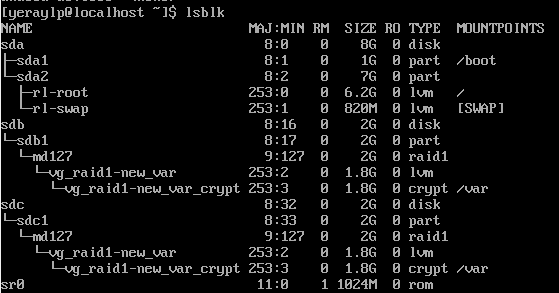
\includegraphics[scale=0.6]{ubuntuRAID.png}
	\caption{Configuración inicial}
\end{figure}

Comprobamos nuestra configuración de RAID con el comando mdadm \cite{mdadm}
\begin{minted}{shell}
$$ sudo mdadm --query /dev/md0 #md127, si el SO lo reasigna
$$ sudo mdadm --detail /dev/md0 #Para mas detalle
\end{minted}
\begin{figure}[H]
	\centering
	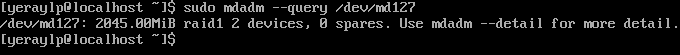
\includegraphics[scale=0.6]{query.png}
\end{figure}

\begin{figure}[H]
	\centering
	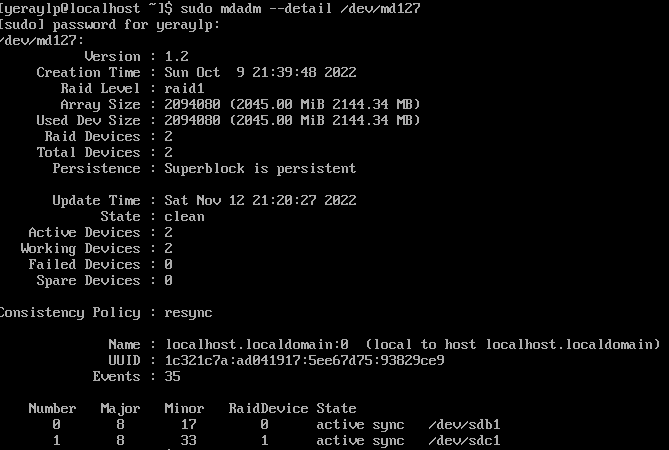
\includegraphics[scale=0.5]{detail.png}
\end{figure}

\code{/proc/mdstat} nos muestra el estado del multidevice:

\begin{figure}[H]
	\centering
	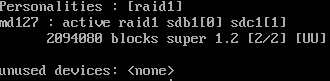
\includegraphics[scale=0.6]{multidevice.png}
	\caption{Más información de mdstat en la doc\cite{mdstat}}
\end{figure}

Lo que nos interesa del fichero es:
\begin{itemize}
	\item U representa un disco encendido(Up) 
	\item \_ representa un disco caído
\end{itemize}
Dos U significa que tenemos 2 discos corriendo.

\subsection{Testear el RAID forzando un fallo vía software (Rocky Linux)}
\begin{minted}{shell}
$$ mdadm --manage --set-faulty /dev/md0 /dev/sdb1 #Tiramos el disco 1 (su unica partición)
\end{minted}

\begin{figure}[H]
	\centering
	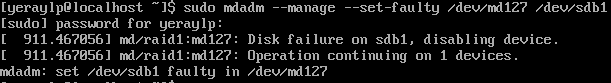
\includegraphics[scale=0.65]{faulty.png}
\end{figure}

En \code{lsblk} no aparece ningún cambio pero sí con los comandos:

\begin{minted}{shell}
$$ sudo mdadm --detail /dev/md127 #OJO --query no muestra nada
$$ cat /proc/mdstat
\end{minted}
\begin{figure}[H]
	\centering
	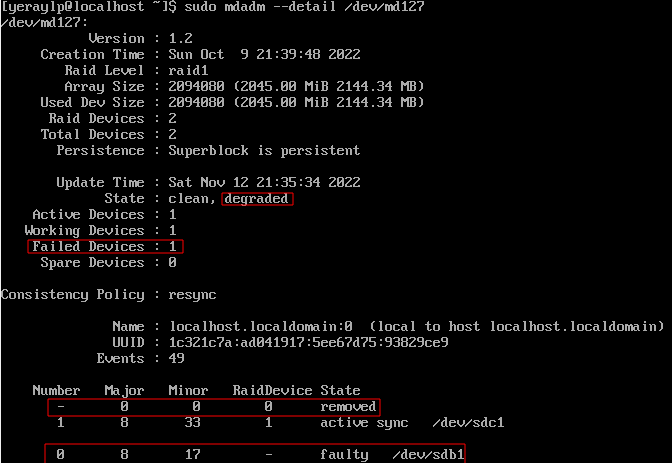
\includegraphics[scale=0.6]{faultystat.png}
	\caption{En rojo podemos ver los cambios al fallar el disco}
\end{figure}
\begin{figure}[H]
	\centering
	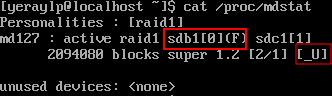
\includegraphics[scale=0.65]{faultyproc.png}
	\caption{La barra baja (\_) nos muestra el disco caído}
\end{figure}

Para recuperar el estado del RAID hay que sacar el disco del mismo RAID y volver a meterlo:
\begin{minted}{shell}
$$ sudo mdadm -r /dev/md0 /dev/sdb1 #Quitamos
$$ cat /proc/mdstat #Comprobamos
$$ sudo mdadm -a /dev/md0 /dev/sdb1 #Añadimos
$$ cat /proc/mdstat #Monitorizamos la recuperacion
\end{minted}
\begin{figure}[H]
	\centering
	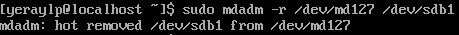
\includegraphics[scale=0.65]{hotremoved.png}
\end{figure}
\begin{figure}[H]
	\centering
	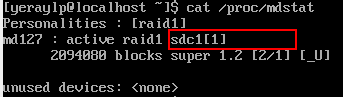
\includegraphics[scale=0.65]{nosdb1.png}
	\caption{Ya no aparece sdb1}
\end{figure}
\begin{figure}[H]
	\centering
	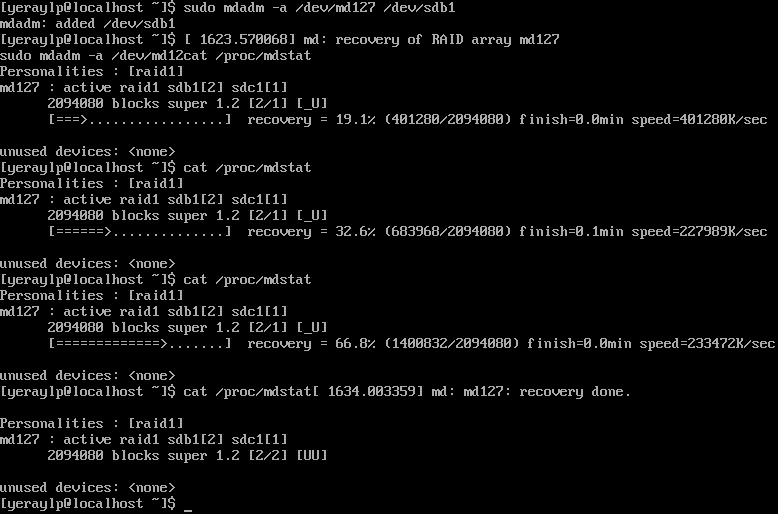
\includegraphics[scale=0.7]{RAIDrecover.png}
\end{figure}

Se puede monitorizar la recuperación del disco con \code{watch}:
\begin{minted}{shell}
watch -n 1 /proc/mdstat #Se sale con Ctrl+C
\end{minted}
\begin{figure}[H]
	\centering
	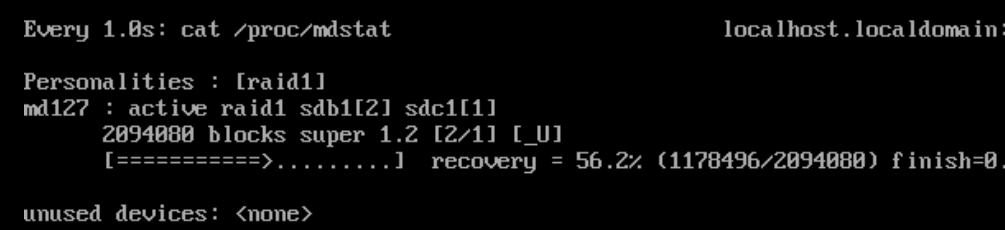
\includegraphics[scale=0.4]{watch.png}
\end{figure}

\subsection{Testear el RAID forzando un fallo vía hardware (Ubuntu)}
Ahora en Ubuntu procederemos a extraer un disco físico como si estuviera defectuoso. Lo quitamos desde la virtualbox:
\begin{figure}[H]
	\centering
	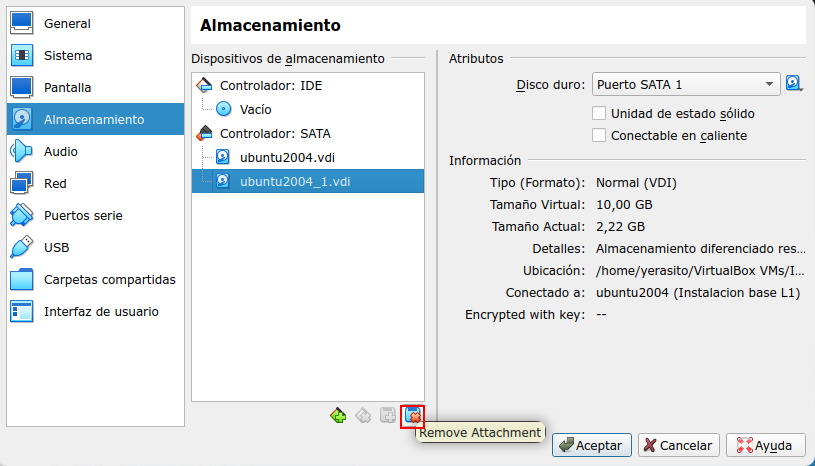
\includegraphics[scale=0.5]{byedisco.png}
\end{figure}

Nos vamos a nuestra máquina y la arrancamos. Nos encontramos el mensaje:

\begin{figure}[H]
	\centering
	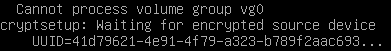
\includegraphics[scale=0.7]{cryptsetup.png}
	\caption{Intenta cargar el disco que hemos quitado, esperamos a que pase el time out.}
\end{figure}

Pasados los 5 minutos nos arrancará el initramfs
\begin{figure}[H]
	\centering
	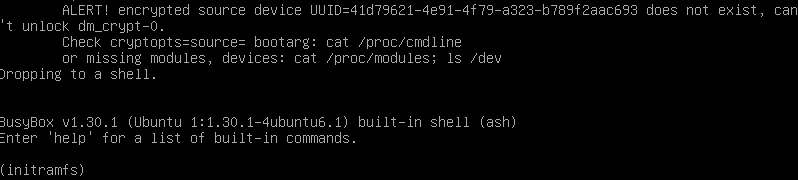
\includegraphics[scale=0.55]{initramfs.png}
\end{figure}

Si nos distrajimos al principio y no vimos el arranque del sistema podemos verlo con el comando \code{dmesg}:

\begin{figure}[H]
	\centering
	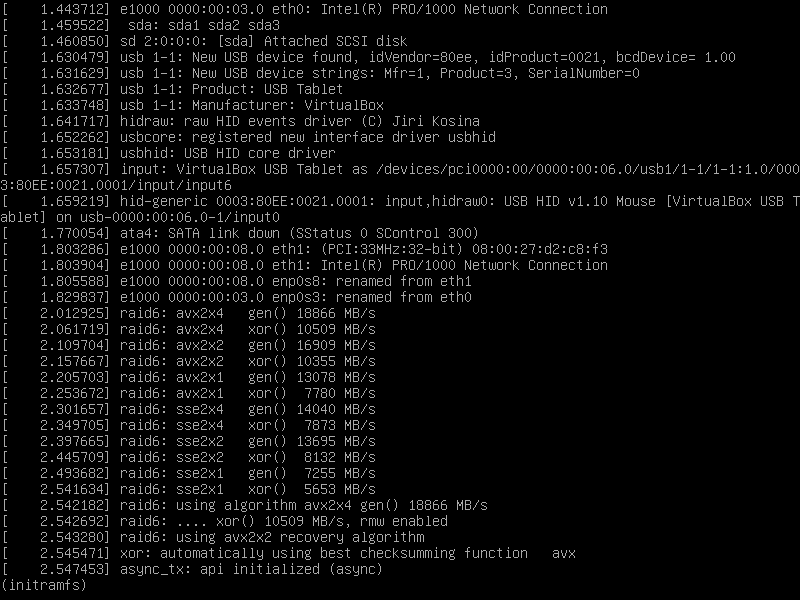
\includegraphics[scale=0.7]{dmesg.png}
\end{figure}

Para depurar el error vamos a mirar en lvm:
\begin{figure}[H]
	\centering
	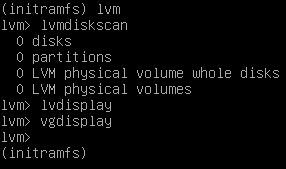
\includegraphics[scale=0.6]{lvm.png}
\end{figure}
No hay información relevante. Miramos ahora en mdstat: 
\begin{figure}[H]
	\centering
	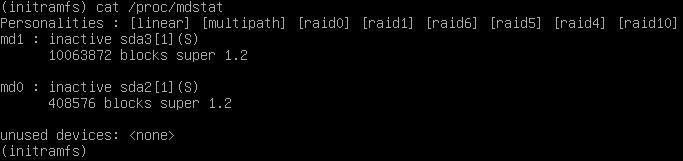
\includegraphics[scale=0.6]{mdstat.png}
\end{figure}

Arrancar ha arrancado el disco pero aparece inactivo. Intentamos activarlo mirando en la documentación de mdstat \cite{mdstat}.

\begin{figure}[H]
	\centering
	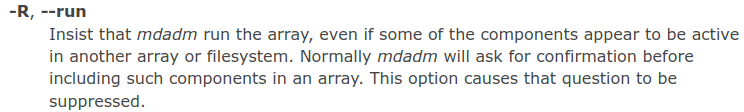
\includegraphics[scale=0.5]{RUN.png}
\end{figure}

Forzamos la activación del \high{md0} y \high{md1}:

\begin{minted}{shell}
$$ mdadm -R /dev/md0
$$ cat /proc/mdstat
$$ mdadm -R /dev/md1
$$ cat /proc/mdstat
#Esperamos un poco a que se terminen de activar y hacemos Ctrl+D para continuar
\end{minted}
\begin{figure}[H]
	\centering
	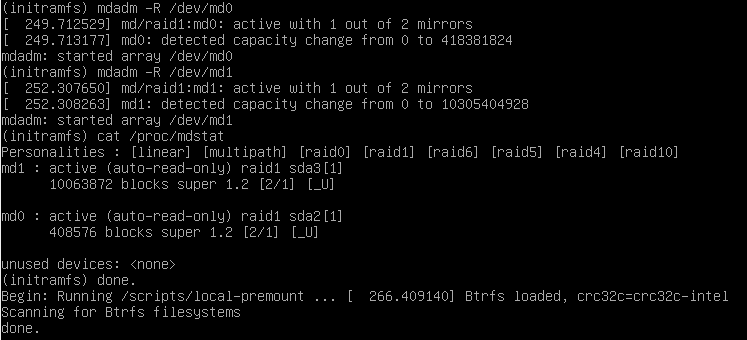
\includegraphics[scale=0.55]{runmd.png}
\end{figure}
Ya entramos a nuestro sistema, lo primero que vamos a hacer es un \code{lsblk}:
\begin{figure}[H]
	\centering
	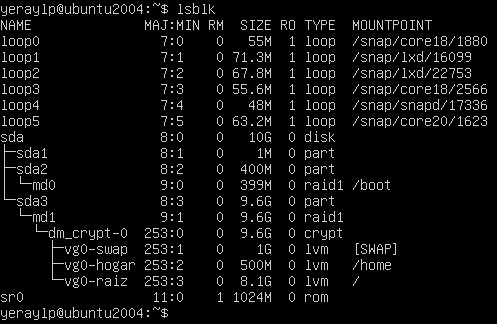
\includegraphics[scale=0.5]{lsblk.png}
	\caption{Hemos arrancado con un único disco}
\end{figure}

\high{IMPORTANTE}: No debemos dar servicio tal y como está el sistema pues con el cliente hemos establecido un contrato donde le servimos RAID 1. Además si se fastidia sda tenemos un serio problema (*aparece el hombre de negro con el maletín*)
\\ \\
Añadimos un nuevo disco en la vm:
\begin{figure}[H]
	\centering
	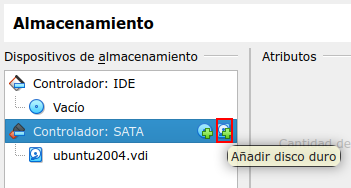
\includegraphics[scale=0.5]{addisk.png}
\end{figure}
\begin{figure}[H]
	\centering
	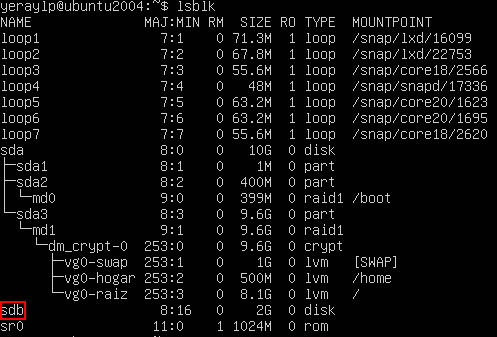
\includegraphics[scale=0.51]{nuevodisco.png}
	\caption{Vuelve sdb}
\end{figure}

Particionamos el disco con \code{fdisk}:

Ojo: al hacer la primera partición debe ser igual que la md0 de sda o nos dará error. En nuestro caso es de \high{+400M}.
\begin{figure}[H]
	\centering
	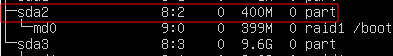
\includegraphics[scale=0.6]{400M.png}
\end{figure}
\begin{figure}[H]
	\centering
	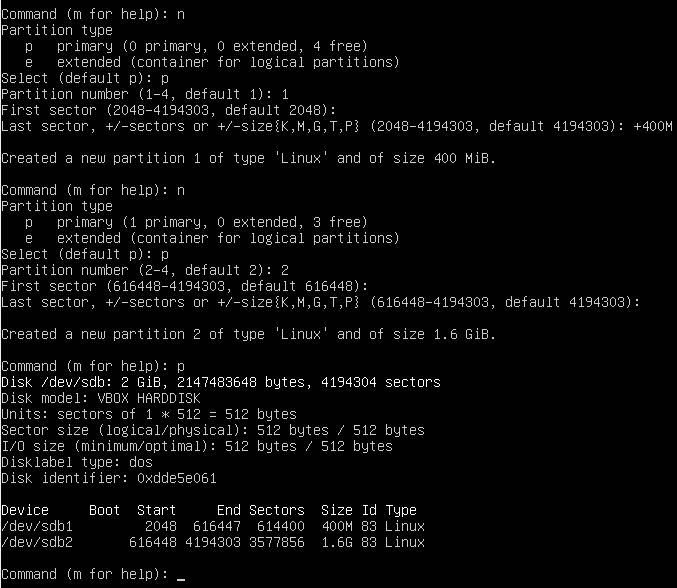
\includegraphics[scale=0.6]{diskpartition.png}
\end{figure}

Instalamos el GRUB en el nuevo disco con: \code{sudo grub-install /dev/sdb}
\begin{figure}[H]
	\centering
	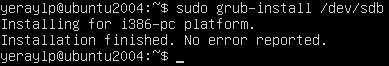
\includegraphics[scale=0.6]{grubinstall.png}
\end{figure}

Añadimos el disco al RAID:
\begin{minted}{shell}
$$ sudo mdadm -a /dev/md0 /dev/sdb1
$$ sudo mdadm -a /dev/md1 /dev/sdb2
$$ watch -n 1 cat /proc/mdstat
\end{minted}

\begin{figure}[H]
	\centering
	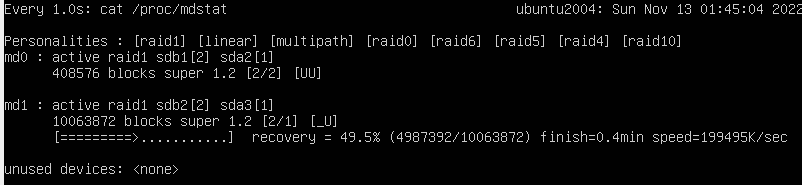
\includegraphics[scale=0.52]{watch2.png}
\end{figure}
Ya tenemos nuestro \high{RAID} de vuelta:

\begin{figure}[H]
	\centering
	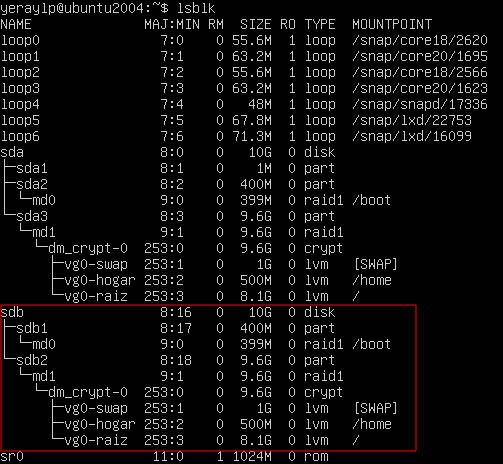
\includegraphics[scale=0.6]{finallsblk.png}
	\caption{En rojo vemos el disco recuperado}
\end{figure}

\section{Instalación y configuración de ZABBIX}
El enunciado práctico dice así: \\
\fbox{\parbox{\textwidth}{\textbf{Ejercicio 1:} \\
		Realice una instalación de ZABBIX 5.0 en su servidor con Ubuntu Server20.04 y configure
		para que se monitorice a él mismo y para que monitorice a la máquina con CentOS.
		Puede configurar varios parámetros para monitorizar, uso de CPU, memoria, etc. pero
		debe configurar de manera obligatoria la monitorización de los servicios SSH y HTTP.
		Documente el proceso de instalación y configuración indicando las referencias que ha
		utilizado así como los problemas que ha encontrado. Para ello, se le recomienda utilizar
		la plantilla de LATEX disponible en SWAD. Procure que en las capturas aparezca su
		nombre de usuario (en el prompt p.ej. como hemos hecho en los exámenes). El archivo
		debe estar subido a SWAD (zona mis trabajos) antes del final del curso (ver actividad
		en SWAD).}}
%------------------------------------------------

\subsection{Instalación del servidor ZABBIX en Ubuntu Server}
Para la instalación del servidor iremos a la guia de instalación oficial de ZABBIX \cite{guiaInstalacion}.
 Para Ubuntu la configuración debe ser la siguiente:
 
\begin{figure}[H]
	\centering
	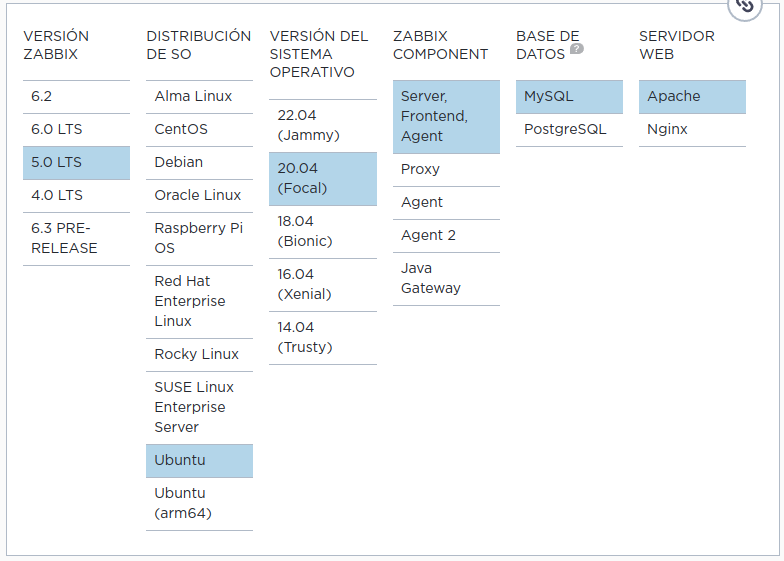
\includegraphics[scale=0.5]{ubuntuZABBIXweb.png}
	\caption{Configuración para ejercicio \cite{zabbixUbuntu}} \label{fig:guiaInstalacion}
\end{figure}
Es recomendable conectarse por ssh a Ubuntu para copiar los comandos de la web de \high{ZABBIX}: \code{ssh yeraylp@192.168.56.105}

\begin{enumerate}
	\item Añadimos el repositorio de ZABBIX:
\begin{minted}{shell}
$$ wget https://repo.zabbix.com/zabbix/5.0/ubuntu/pool/main/z/zabbix
-release/zabbix-release_5.0-1%2Bfocal_all.deb
$$ sudo dpkg -i zabbix-release_5.0-1+focal_all.deb
$$ sudo apt update
\end{minted}
\begin{figure}[H]
	\centering
	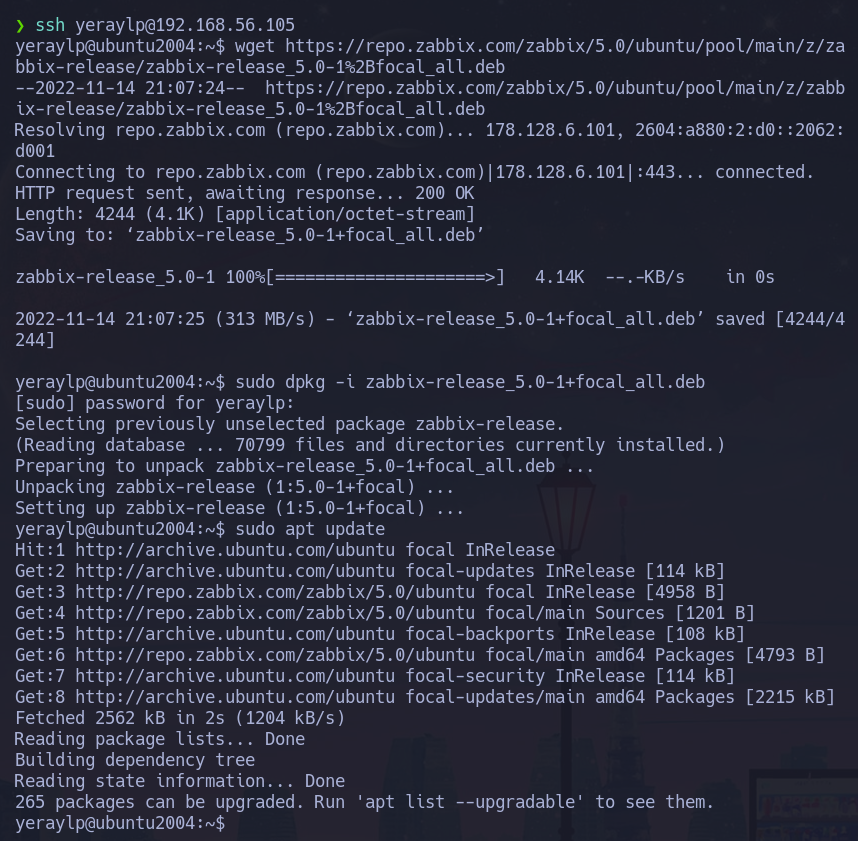
\includegraphics[scale=0.45,right]{repoadd.png} 
\end{figure}
	
	\item Instalamos el servidor, el front-end y el agente:
\begin{minted}{shell}
$$ sudo apt install zabbix-server-mysql zabbix-frontend-php zabbix-apache-conf zabbix-agent
\end{minted}

\item Instalamos mysql y creamos la base de datos de ZABBIX:
\begin{minted}{bash}
$$ sudo apt install mysql-server
$$ sudo mysql_secure_installation #Securizar mysql
$$ sudo mysql -uroot -p
\end{minted}

\begin{minted}{sql}
mysql> create database zabbix character set utf8 collate utf8_bin;
mysql> create user zabbix@localhost identified by 'practicas,ISE';
mysql> grant all privileges on zabbix.* to zabbix@localhost;
mysql> quit;
\end{minted}

\begin{figure}[H]
	\centering
	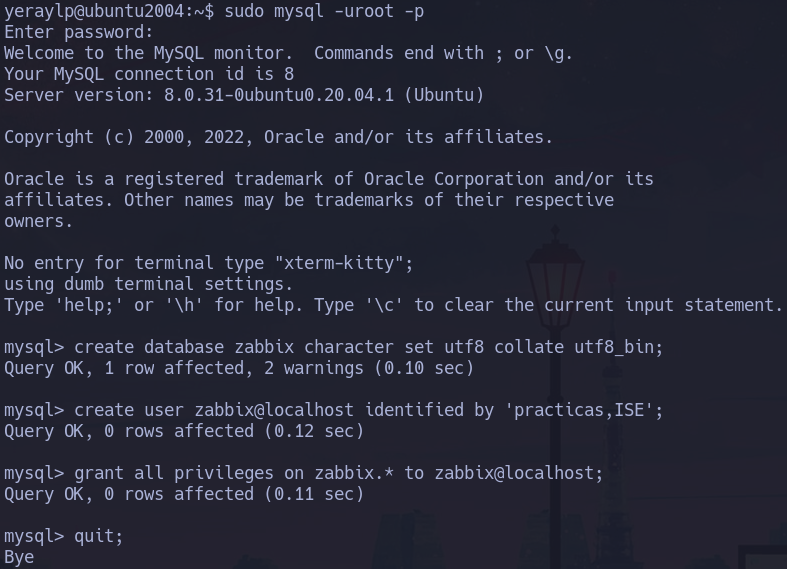
\includegraphics[scale=0.5,right]{mysql.png} 
\end{figure}

	\item Importamos el esquema y los datos al servidor de ZABBIX. \\
	Nota: \code{-pzabbix} indica que la contraseña es zabbix. \code{-p zabbix} indica que la contraseña se mete por prompt y zabbix es la base de datos por defecto.
	\begin{minted}{shell}
$$ sudo zcat /usr/share/doc/zabbix-server-mysql*/create.sql.gz | mysql -uzabbix -p zabbix
	\end{minted}
Tarda un buen rato (5-10 min).

\begin{figure}[H]
	\centering
	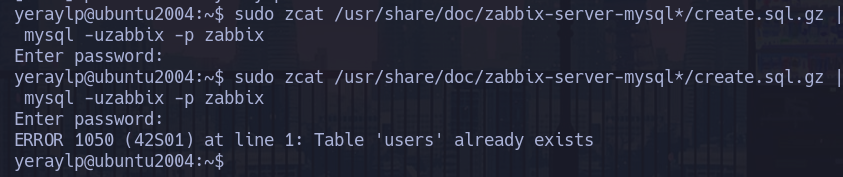
\includegraphics[scale=0.46,right]{zcat.png} 
	\caption{Al ejecutar de nuevo el comando nos avisará de que ya está creado}
\end{figure}

	\item Configuramos la contraseña en la base de datos. Para ello accedemos a: \\ \code{/etc/zabbix/zabbix\_server.conf}, buscamos /DBPassword, lo descomentamos y ponemos la clásica contraseña \code{practicas,ISE}
\begin{figure}[H]
	\centering
	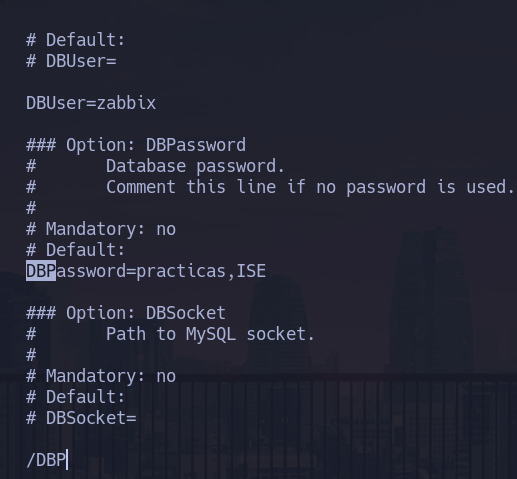
\includegraphics[scale=0.46,center]{dbpassword.png} 
\end{figure}

\item Configuramos PHP para el front-end de zabbix. Para ello accedemos a: \\
\code{/etc/zabbix/apache.conf} y descomentamos las dos lineas de date.timezone. \\
$[$Opcional$]$ Cambiar Riga por Madrid

\begin{figure}[H]
	\centering
	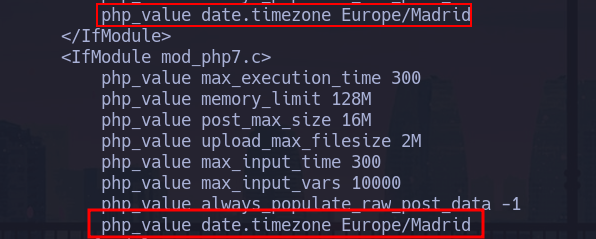
\includegraphics[scale=0.46,center]{timezone.png} 
\end{figure}

	\item Reiniciamos y habilitamos los servicios
	\begin{minted}{shell}
$$ sudo systemctl restart zabbix-server zabbix-agent apache2
$$ sudo systemctl enable zabbix-server zabbix-agent apache2
$$ sudo systemctl status zabbix-server zabbix-agent apache2
	\end{minted}

\begin{figure}[H]
	\centering
	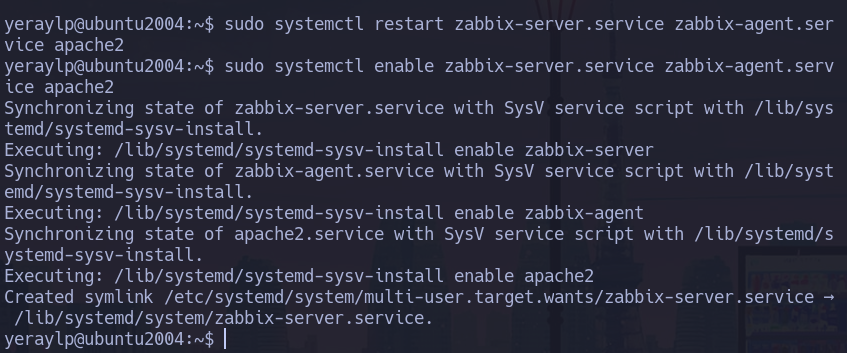
\includegraphics[scale=0.46,right]{systemdzabbix.png} 
\end{figure}

\end{enumerate}


%----------------------------------------------------------------------------------------
%	Cuestión 2
%----------------------------------------------------------------------------------------

\subsection{Configuración del servidor (Ubuntu)}

A partir de aquí usaremos la guía de \href{https://www.zabbix.com/documentation/5.0/en/manual/quickstart/login}{inicio rápido}.

\begin{enumerate}
	\item Ejecutar el setup de zabbix a través de un navegador. Abrimos: \\
	\url{http://192.168.56.105/zabbix/setup.php}
	\begin{figure}[H]
		\centering
		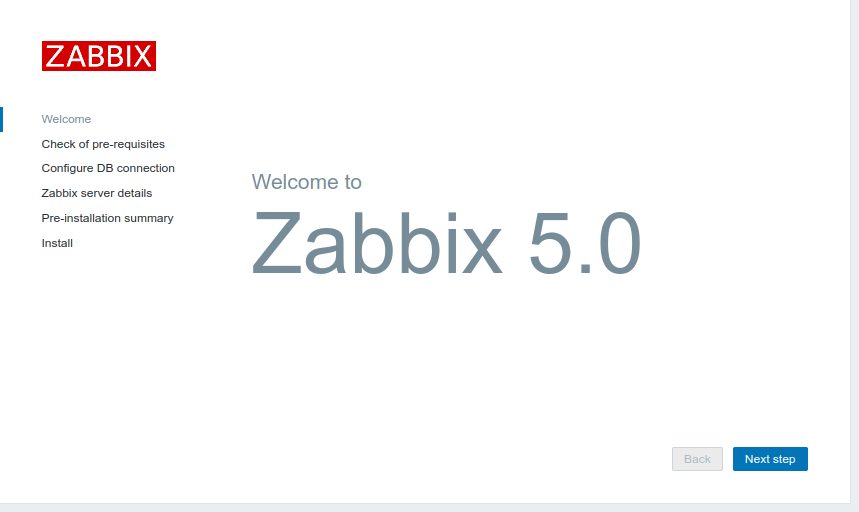
\includegraphics[scale=0.46,center]{welcome.png} 
	\end{figure}

	\item Al pasar al siguiente paso veremos que nos dará error la date.timezone de PHP:
	\begin{figure}[H]
		\centering
		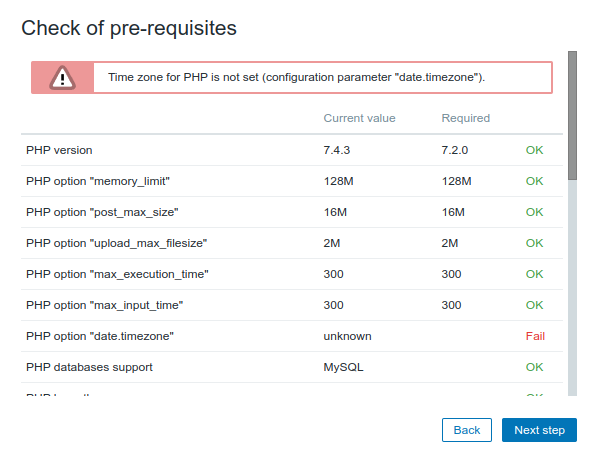
\includegraphics[scale=0.46,center]{phptimezone.png} 
	\end{figure}
Para arreglarlo, nos vamos a \code{/etc/php/7.4/apache2/php.ini} y descomentamos la linea: \code{date.timezone}:
	\begin{figure}[H]
	\centering
	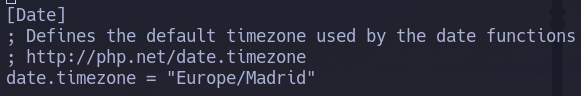
\includegraphics[scale=0.46,center]{phpfix.png} 
	\end{figure}
Reiniciamos el servicio apache2: \code{sudo systemctl restart apache2}
	\begin{figure}[H]
	\centering
	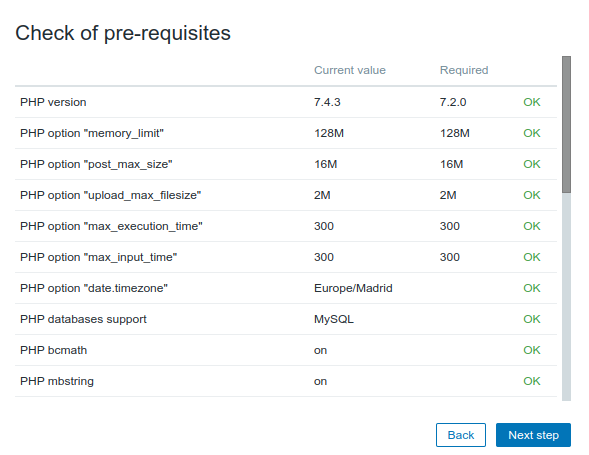
\includegraphics[scale=0.47,center]{checkPrerrequisitos.png} 
	\end{figure}

	\item Configuramos la conexión a la base de datos. Dejamos todo por defecto y ponemos la mítica contraseña: \code{practicas,ISE}
	\begin{figure}[H]
	\centering
	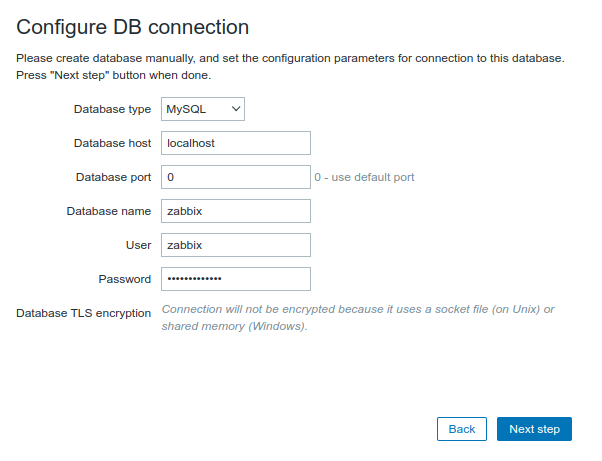
\includegraphics[scale=0.55,center]{configuredb.png} 
	\end{figure}
	
	\item Dejamos el puerto del servidor por defecto:
	\begin{figure}[H]
	\centering
	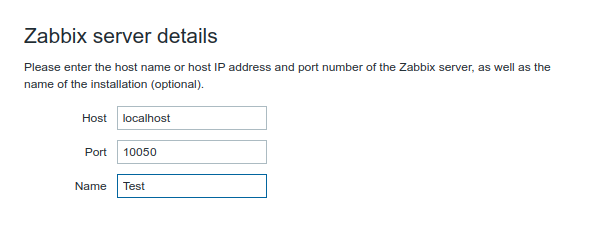
\includegraphics[scale=0.6,center]{defaultport.png} 
	\end{figure}

	\item Listo! El servidor ya está configurado
	\begin{figure}[H]
	\centering
	
\includegraphics[scale=0.65,center]{successful.png} 
	\end{figure}
\end{enumerate}

%----------------------------------------------------------------------------------------
%	Cuestión 3
%----------------------------------------------------------------------------------------

\subsection{Configuración del agente (Ubuntu) [opcional]}
Esta parte no es realmente necesaria pues podemos monitorizar Ubuntu directamente desde el servidor. La ventaja de separarlos es que podemos añadir específicamente los items que queramos al host.\\

Para acceder al servidor de zabbix nos vamos a: \url{http://192.168.56.105/zabbix/} y nos logeamos con las siguientes credenciales por defecto:
	\begin{figure}[H]
	\centering
	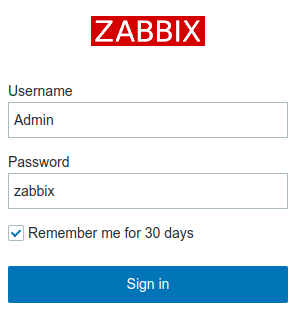
\includegraphics[scale=0.75,center]{loginzabbix.png} 
	\end{figure}
Una vez accedemos nos encontramos con la dashboard:
	\begin{figure}[H]
	\centering
	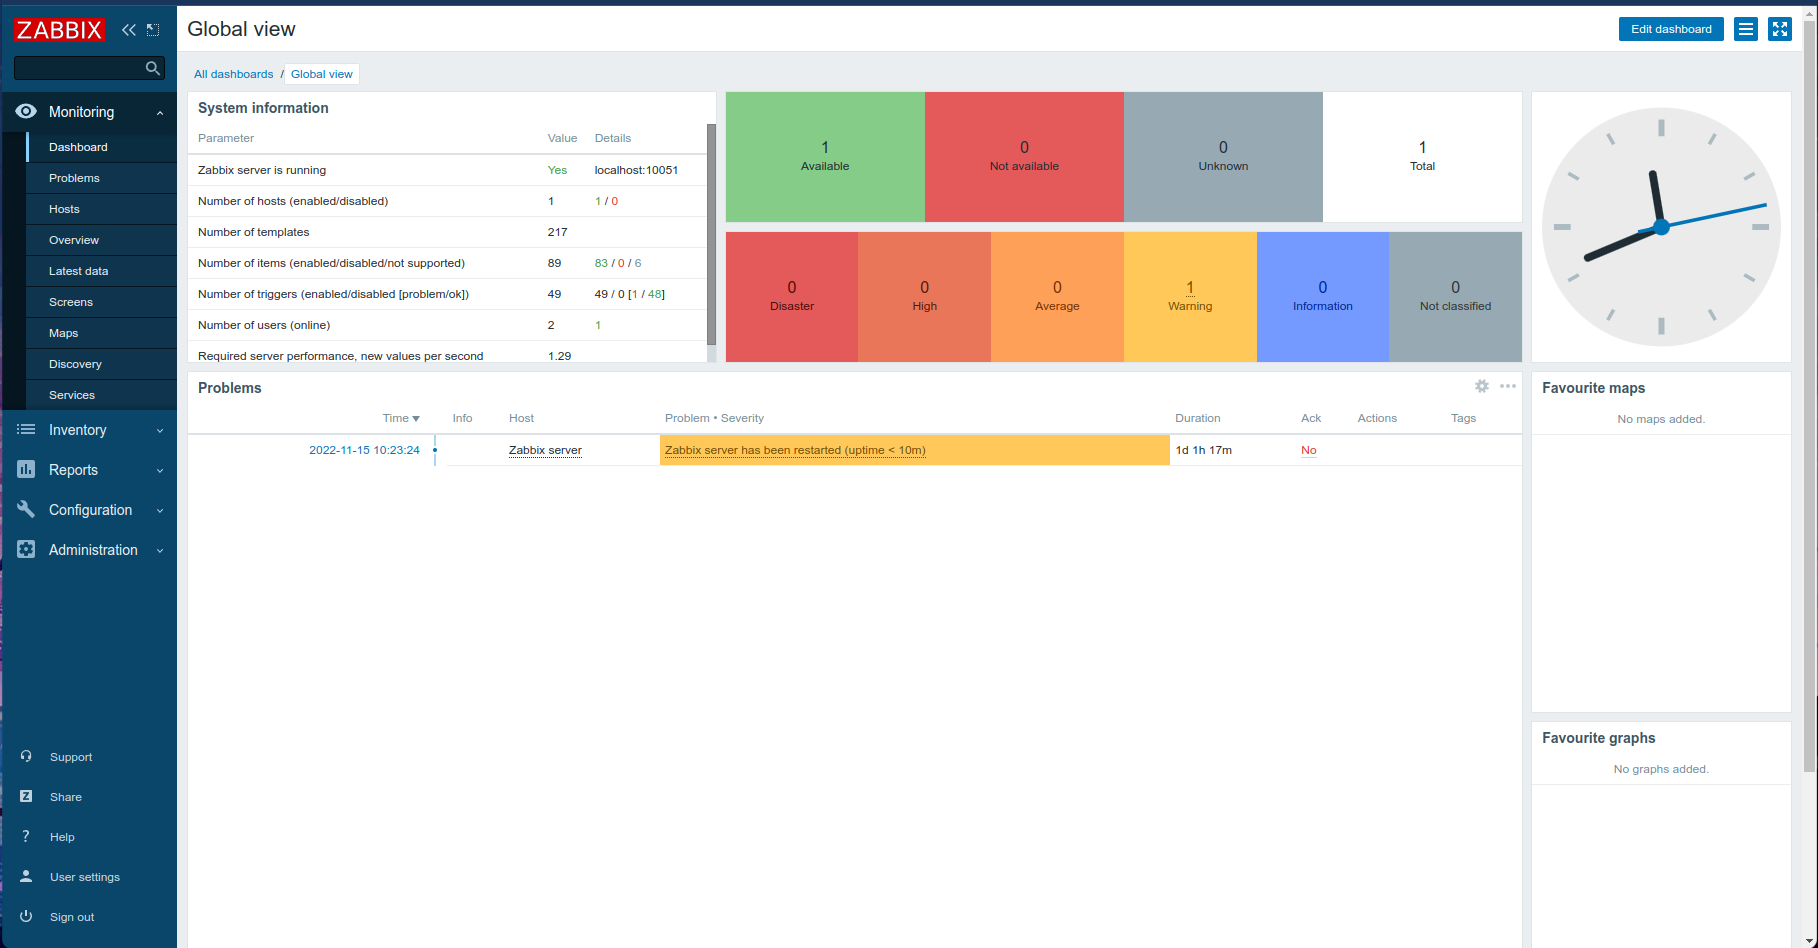
\includegraphics[scale=0.23,center]{dashboard.png} 
	\caption{Aquí veremos los problemas que surjan de los hosts}
	\end{figure}

Para “monitorizar” cualquier servicio tenemos que ir a: 
\dirtree{%
.1 Monitoring.
.2 Latest data.
.3 Host Rocky Linux.
.3 ISE Host (Ubuntu zabbix-agent).
.3 Zabbix server (Ubuntu zabbix-server).
}
Seleccionamos el host que queramos monitorizar:
	\begin{figure}[H]
	\centering
	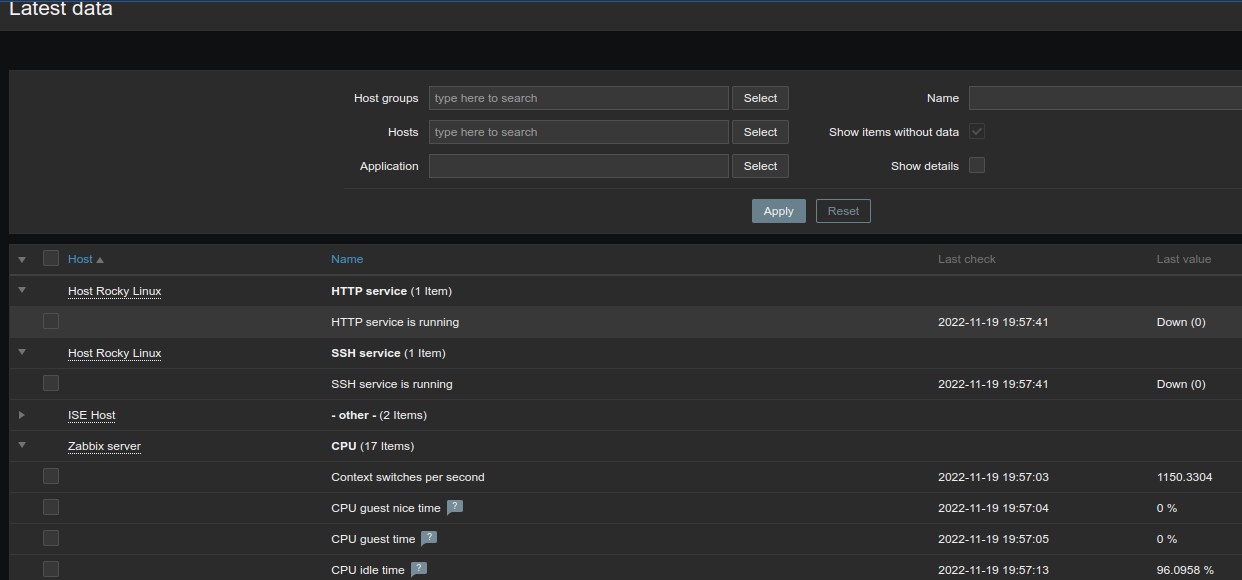
\includegraphics[scale=0.40,center]{latestdata.png} 
	\end{figure}

Sin embargo lo que nos piden es monitorizar el servicio SSH y HTTP. Para ello vamos a configurar el agente en nuestro servidor:

\begin{itemize}
	\item Vamos al archivo de configuración del agente: \code{/etc/zabbix/zabbix\_agentd.conf}. Buscamos \high{/server}. \\
	Server se encarga de las comprobaciones pasivas (servidor al agente). Son las IPs que acepta el agente.
	
	\begin{figure}[H]
	\centering
	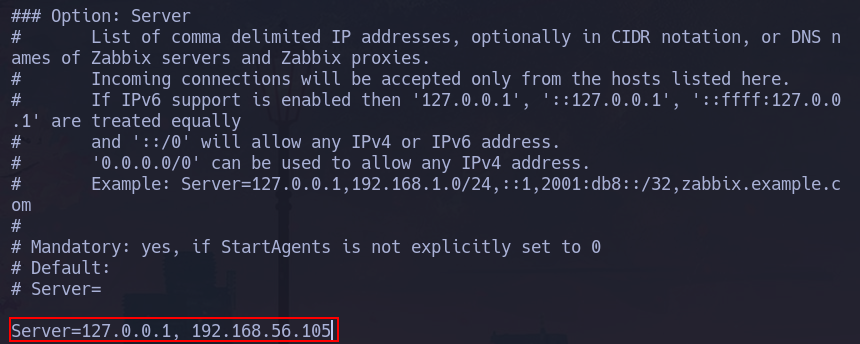
\includegraphics[scale=0.45,right]{agentserver.png} 
	\end{figure}

Añadimos un nuevo host cambiando el HostName en el \code{.conf} y lo creamos desde la web de zabbix:
	\begin{figure}[H]
		\centering
		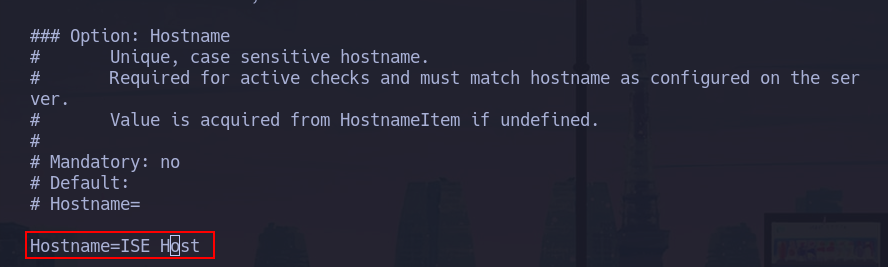
\includegraphics[scale=0.4,right]{ubuhostname.png} 
	\end{figure}
	\begin{figure}[H]
	\centering
	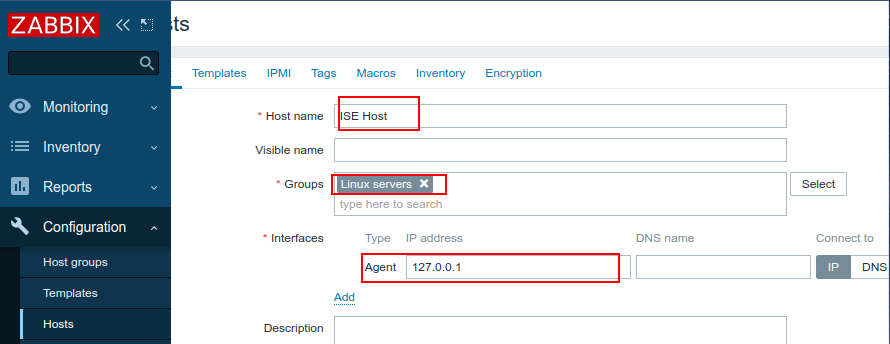
\includegraphics[scale=0.4,right]{ubuhostname2.png} 
	\end{figure}
\end{itemize}
Reiniciamos el servicio: \code{systemctl restart zabbix-agent} y listo, todo configurado.

\subsection{Instalar agente ZABBIX (Rocky Linux)}
Para la instalación del agente de zabbix en Rocky volveremos a la página de instalación \cite{zabbixRocky}

\begin{figure}[H]
	\centering
	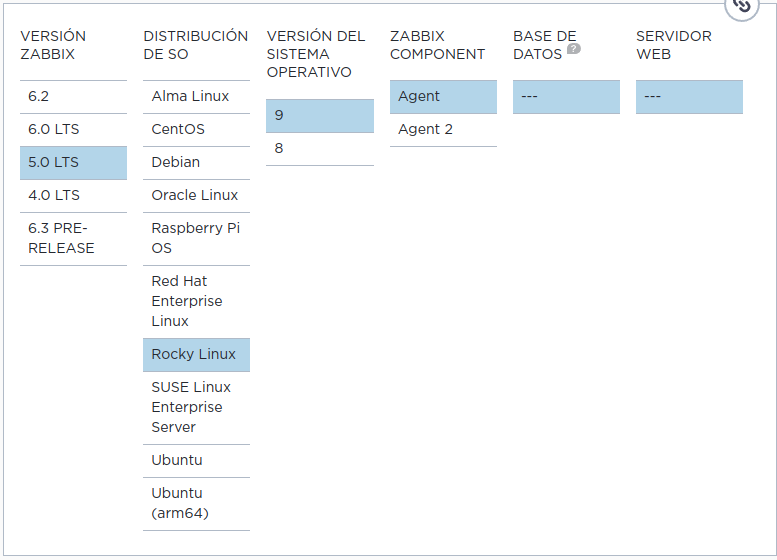
\includegraphics[scale=0.42,center]{rockyZABBIXweb.png} 
\end{figure}

\begin{enumerate}
	\item Añadimos el repositorio de zabbix
	\begin{minted}{shell}
$$ sudo rpm -Uvh https://repo.zabbix.com/zabbix/5.0/rhel/9/x86_64/zabbix-release-5.0-3.e
l9.noarch.rpm
$$ dnf clean all
	\end{minted}
\begin{figure}[H]
	\centering
	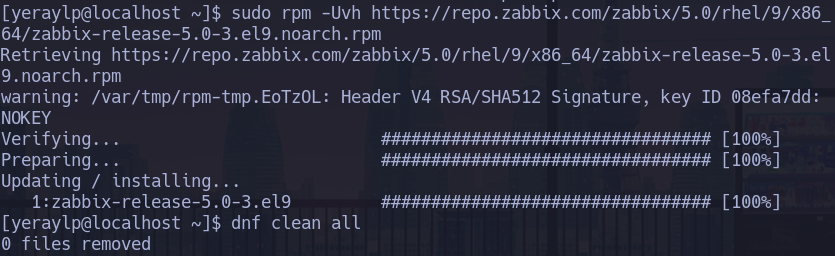
\includegraphics[scale=0.47,right]{rockyrepo.png} 
\end{figure}

	\item Instalamos el agente
	\begin{minted}{shell}
$$ dnf install zabbix-agent
	\end{minted}

	\item Modificamos el fichero de configuración del agente
	\begin{minted}{shell}
$$ sudo vi /etc/zabbix/zabbix_agentd.conf
	\end{minted}
\begin{minted}{shell}
Server=192.168.56.110 #Ip del agente(Rocky)
HostName=Host Rocky Linux
\end{minted}
	\item Reiniciamos y habilitamos el agente
	\begin{minted}{shell}
$$ sudo systemctl restart zabbix-agent
$$ sudo systemctl enable zabbix-agent
	\end{minted}

	\item Creamos un host. Nos vamos al navegador: \url{http://192.168.56.105/zabbix/} \\
\begin{minipage}{4cm}
	\dirtree{%
		.1 Configuration.
		.2 Hosts.
		.3 Create Host.
	}
\end{minipage}

En la interfaz del agente ponemos la IP de Rocky:
\begin{figure}[H]
	\centering
	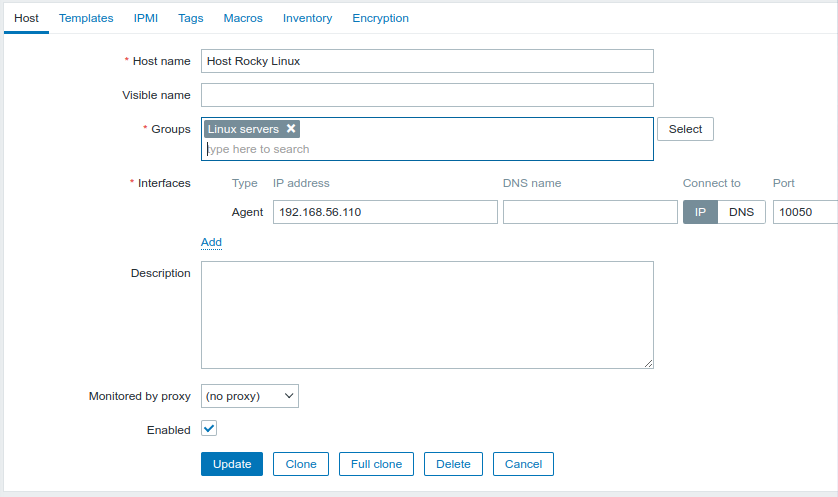
\includegraphics[scale=0.5,right]{rockyhost.png} 
\end{figure}

\end{enumerate}

CUIDADO: para monitorizar los servicios en Rocky linux es necesario habilitar los puertos de los servicios \high{ssh} y \high{http} en el cortafuegos
\begin{minted}{shell}
$$ sudo firewall-cmd --add-port=22/tcp --permanent
$$ sudo firewall-cmd --add-port=80/tcp --permanent
$$ sudo firewall-cmd --add-port=10050/tcp --permanent
$$ sudo firewall-cmd --reload
\end{minted}

\subsection{Monitorización}
En esta sección veremos como podemos comprobar, detectar y corregir incidencias gracias a las herramientas que ofrece ZABBIX.
\subsubsection{Creación y configuración de items}
Para monitorizar el \high{ssh} y \high{http} tenemos 2 opciones: Usar \textit{Templates} o añadir los items a mano. Ambas formas son válidas siempre y cuando en los templates modifiquemos el puerto correspondiente y entendamos como funcionan. Lo vamos a hacer de las dos maneras.
\subsubsection{Templates}
En esta subsección añadiremos los servicios al monitor mediante templates. Para ello:
\begin{enumerate}
	\item Tenemos que ir a: \\
	\begin{minipage}{4cm}
		\dirtree{%
		.1 Configuration.
		.2 Hosts.
		.3 ISE Host.
		}
	\end{minipage} \\
Pinchamos sobre nuestro host \high{ISE Host} y nos vamos al apartado de \textit{Templates}.
\\ Desde allí añadimos los templates \high{SSH} y \high{HTTP} service:
\begin{figure}[H]
	\centering
	\includegraphics[scale=0.47,right]{templates.png} 
\end{figure}

	\item Una vez creados, para añadir el puerto vamos a: \\
	\begin{minipage}{10cm}
	\dirtree{%
		.1 Configuration.
		.2 Templates.
		.3 Template App (ssh o http) Service.
	}
\end{minipage} \\
En name buscamos la plantilla que queremos modificar y le damos a Items:
\begin{figure}[H]
	\centering
	\includegraphics[scale=0.42,center]{iraitemtemplate.png} 
\end{figure}

	\item Pinchamos en el nombre del item:
\begin{figure}[H]
	\centering
	\includegraphics[scale=0.51,center]{itemname.png} 
\end{figure}

	\item Añadimos el puerto \code{net.tcp.service[ssh,,22]} y \code{net.tcp.service[http,,80]} respectivamente.

\begin{figure}[H]
	\centering
	\includegraphics[scale=0.47,right]{sshport.png} 
	\includegraphics[scale=0.644,right]{httport.png} 
\end{figure}
\end{enumerate}

\subsubsection{Añadir items a mano}
Vamos a: \\
\dirtree{%
	.1 Configuration.
	.2 Hosts.
	.3 ISE Host.
	.4 Items.
}

\begin{enumerate}
	\item Creamos un nuevo item:
\begin{figure}[H]
	\centering
	\includegraphics[scale=0.322,right]{createitem.png} 	
\end{figure}
\begin{figure}[H]
	\centering
	\includegraphics[scale=0.495,right]{additem.png} 
\end{figure}

	\item Para saber que key poner recurrimos a la documentación de zabbix: 
\begin{figure}[H]
	\centering
	\includegraphics[scale=0.4,right]{zabbixkey.png} 
	\caption{Extracto del apartado de keys de zabbix \cite{zabbixKeys}}
\end{figure}
Debemos poner: 
%java es por verlo mejor
\begin{minted}{java}
net.tcp.service[ssh,,22]
net.tcp.service[http,,80]
\end{minted}
	\begin{itemize}
		\item Creamos el item para ssh
		\begin{figure}[H]
			\centering
			\includegraphics[scale=0.52,right]{sshitem.png} 
		\end{figure}
		\item Creamos el item para http
		\begin{figure}[H]
			\centering
			\includegraphics[scale=0.52,right]{httpitem.png} 
		\end{figure}
	\end{itemize}

\end{enumerate}

\subsection{Monitoreo en la web de zabbix}
Si tiramos un servicio, por ejemplo, el ssh: \code{sudo systemctl stop sshd} y esperamos unos minutos.
Veremos que nos indica un problema:
		\begin{figure}[H]
		\centering
		\includegraphics[scale=0.495,right]{problemnotification.png} 
		\end{figure}
Si nos vamos a: \\
\dirtree{%
	.1 Monitoring.
	.2 Problems.
}
\begin{figure}[H]
	\centering
	\includegraphics[scale=0.45,right]{problemstatus.png}
	\caption{Tenemos un problema de severidad media desde las 13:04:38}
\end{figure}

Si le damos al tiempo veremos más detalles:
\begin{figure}[H]
	\centering
	\includegraphics[scale=0.495,right]{problemdetail.png} 
\end{figure}

Si volvemos al apartado de problemas y pinchamos sobre SSH service is down, veremos el siguiente cuadro:
\begin{figure}[H]
	\centering
	\includegraphics[scale=0.495,center]{problemcuadro.png} 
\end{figure}

Al pulsar en debajo de HISTORY podemos ver la gráfica:
	\begin{figure}[H]
	\centering
	\includegraphics[scale=0.42,center]{graphicdown.png} 
\end{figure}

Cuando encendemos el servicio de nuevo y esperamos 1 min (la tasa de refresco del trigger) vemos que la gráfica vuelve a UP:
\begin{figure}[H]
	\centering
	\includegraphics[scale=0.495,center]{upgraphic.png} 
	\caption{Nuestro servicio está activo de nuevo}
\end{figure}
\begin{figure}[H]
	\centering
	\includegraphics[scale=0.325,right]{resolvedstatus.png} 
	\caption{Problema resuelto}
\end{figure}
Podemos hacer lo mismo con http: \code{sudo systemctl stop apache}
Al hacerlo en Ubuntu la página de ZABBIX se caerá, no pasa nada, esperamos unos minutos y activamos el servicio.

\begin{figure}[H]
	\centering
	\includegraphics[scale=0.45,right]{problemhttp.png} 
\end{figure}
		\begin{figure}[H]
	\centering
	\includegraphics[scale=0.446,right]{resolvedhttp.png} 
\end{figure}

\section{Instalación y configuración de ANSIBLE}
El siguiente enunciado práctico dice así: \\
\fbox{\parbox{\textwidth}{\textbf{Ejercicio 2:} \\
Usted deberá saber cómo instalar y configurar Ansible para poder hacer
un ping a las máquinas virtuales de los servidores y ejecutar un comando básico (p.ej.
el script de monitorización del RAID1). También debe ser consciente de la posibilidad
de escribir acciones más complejas mediante playbooks escritos con YAML como, por
ejemplo, asegurarse de que tenemos la última versión instalada de httpd y que está en
ejecución. Incluya capturas de pantalla del proceso con una breve descripción en el mismo
documento que suba para el ejercicio de Zabbix.}}

\subsection{Instalación}
Para la instalación de la herramienta ansible recurrimos a su página oficial \cite{ansibleinstall}:
\begin{enumerate}
	\item Instalamos ansible:
	\begin{minted}{shell}
$$ sudo apt update
$$ sudo apt install software-properties-common
$$ sudo add-apt-repository --yes --update ppa:ansible/ansible
$$ sudo apt install ansible
	\end{minted}
	
	\item Añadimos las IP de las maquinas virtuales y el usuario que ansible debe usar para logearse en \code{/etc/ansible/hosts}:
	\begin{figure}[H]
		\centering
		\includegraphics[scale=0.5,center]{ansiblehosts.png} 
	\end{figure}

	\item Generamos y añadimos las claves publicas de ambas máquinas para que ansible pueda conectarse vía ssh, incluido localhost.
\begin{minted}{shell}
#En Ubuntu
$$ ssh-keygen
$$ ssh-copy-id 192.168.56.105 #Añadimos la key de Ubuntu a sí mismo
$$ ssh-copy-id 192.168.56.110 # Añadimos la key de Ubuntu a rocky
\end{minted}

\begin{figure}[H]
	\centering
	\includegraphics[scale=0.45,center]{sshkeys.png} 
\end{figure}

	\item Comprobamos que ansible puede conectarse a ambas máquinas haciendo ping
\begin{minted}{shell}
$$ ansible all -m ping
\end{minted}

\begin{figure}[H]
	\centering
	\includegraphics[scale=0.47,center]{ansibleping.png} 
\end{figure}
\end{enumerate}

\subsection{Creación de un inventario \cite{ansibleguide}}
Los inventarios nos permiten agrupar hosts en grupos.
Creamos el fichero: \code{vi inventory.yaml}
\begin{minted}{yaml}
virtualmachines:
   hosts:
      ubuntu2004:
         ansible_host: 192.168.56.105
      rocky:
         ansible_host: 192.168.56.110
\end{minted}

Ahora podemos hacer ping con el nuevo grupo virtualmachines
\begin{figure}[H]
	\centering
	\includegraphics[scale=0.58,center]{inventory.png} 
\end{figure}

\subsection{Creación de un playbook}
Los playbook son listas de tareas que ansible ejecuta de una en una en los servidores que especifiquemos. Se recomienda mirar la documentación de modulos builtin \cite{ansiblebuiltin}.
\\Creamos el fichero: \code{vi playbook.yaml}
\begin{minted}{yaml}
- name: Libro de prueba #Nombre del libro
  hosts: virtualmachines
  task: #Lista de tareas
   - name: Ping a los hosts #1ªTarea
     ansible.builtin.ping:
   - name: Imprime un mensaje #2ªTarea
     ansible.builtin.debug:
        msg: Hello world
\end{minted}

Para ejecutar el libro usamos el comando \code{ansible-playbook}:
\begin{minted}{shell}
$$ ansible-playbook -i inventory.yaml playbook.yaml
\end{minted}
\begin{figure}[H]
	\centering
	\includegraphics[scale=0.48,center]{playbook.png} 
\end{figure}

\subsection{Comprobar los RAIDs de los servidores}
Creamos el fichero \code{monitorRAIDs.py}:
\begin{minted}{python}
import re
import sys
f=open('/proc/mdstat')
for line in f:
    b=re.findall('\[[U]*[_]+[U]*\]',line)
    if(b!=[])
        print("---ERROR_en_RAID---")
        sys.exit()
print("---OK_Script---")
\end{minted}
Nota: el script original tenia un error ya que siempre devolvía OK\_Script. Hay que añadir \code{sys.exit()} para devolver error en caso de que un RAID haya fallado. \\

Podemos ejecutar el comando en la shell o en un libro:
\subsubsection{Ejecutando un script en la shell}
Es necesario que el script se encuentre en el mismo directorio en ambos servidores, para ello usamos el comando \code{scp}.

\begin{minted}{shell}
#Copiamos el script de ubuntu a rocky
$$ scp monitorRAIDs.py yeraylp@192.168.56.110:/home/yeraylp/
#Ejecutamos el script con ansible
$$ ansible virtualmachines -m shell -a 'python monitorRAIDs.py' -i inventory.yaml
\end{minted}
\begin{figure}[H]
	\centering
	\includegraphics[scale=0.5,center]{monitorSHELL.png} 
\end{figure}

\subsubsection{Ejecutando un script usando un playbook}
Esta vez basta con que el script se encuentre en el servidor donde se ejecuta el playbook. Creamos el fichero \code{scriptplaybook.yaml}:
\begin{minted}{yaml}
- name: Libro para ejecutar un script
  hosts: virtualmachines
  tasks:
   - name: Ping a los hosts
     ansible.builtin.ping:
   - name: Comprobamos RAIDs con un script de python
     ansible.builtin.script:
        executable: python3
        cmd: monitorRAIDs.py
     register: data
   - name: Imprimir la salida del script
     ansible.builtin.debug:
        var: data.stdout_lines
\end{minted}
Reutilizamos el inventario de antes (o usamos el grupo webservices):
\begin{minted}{yaml}
virtualmachines:
   hosts:
   ubuntu2004:
      ansible_host: 192.168.56.105
   rocky:
      ansible_host: 192.168.56.110
\end{minted}
Y ejecutamos el libro:
\begin{minted}{shell}
$$ ansible-playbook -i inventory.yaml playbook.yaml #Ejecutamos el libro
\end{minted}

\begin{figure}[H]
	\centering
	\includegraphics[scale=0.47,center]{scriptplaybook.png} 
\end{figure}

Si forzamos un error en un RAID, por ejemplo, el de Ubuntu:\\

\begin{minted}{shell}
$$ mdadm --manage --set-faulty /dev/md0 /dev/sdb1 #Tiramos el disco 1
\end{minted}
El script nos mostrará el error:
\begin{figure}[H]
	\centering
	\includegraphics[scale=0.48,center]{faultyplaybook.png} 
\end{figure}

Igual con Rocky:
\begin{figure}[H]
	\centering
	\includegraphics[scale=0.65,center]{rockyfaulty.png} 
\end{figure}
\begin{figure}[H]
	\centering
	\includegraphics[scale=0.55,center]{rockyfaulty2.png} 
\end{figure}
\subsection{Verificar instalación de httpd y su ejecución}
Es demasiado complejo para usarlo en la shell, usamos un playbook. \\
\high{CUIDADO}: no podemos ejecutar la misma key en ambos servidores pues Ubuntu usa \code{apache2} mientras que Rocky usa \code{httpd}.

Creamos el libro con 2 bloques de tareas: \code{vi playbook.yaml}
\begin{minted}{yaml}
- name: Ubuntu comprobar apache
  hosts: ubuntu2004
  become: true
  become_user: root
  tasks:
   - name: comprobar que apache está en su última version
     ansible.builtin.apt:
       name: apache2
       state: latest
   - name: comprobar que apache esta corriendo
     ansible.builtin.systemd:
       name: apache2
       state: started

- name: Rocky comprobar httpd
  hosts: rocky
  become: true
  tasks:
  - name: comprobar que httpd está en su ultima version
    ansible.builtin.dnf:
      name: httpd
      state: latest
 - name: comprobar que http esta corriendo
   ansible.builtin.systemd: 
      name: httpd
      state: started
\end{minted}

Para ejecutar este libro es necesario permisos de administrador, por ello usamos el BECOME user:
\begin{minted}{shell}
$$ ansible-playbook -i inventory.yaml checkplaybook.yaml -K
\end{minted}
\code{-K} MAYÚSCULA nos permite convertirnos en root
\begin{figure}[H]
	\centering
	\includegraphics[scale=0.45,center]{checkhttp.png} 
\end{figure}
Para comprobarlo vamos a eliminar el servicio \code{httpd} en Rocky:
\begin{figure}[H]
	\centering
	\includegraphics[scale=0.7,center]{httpremove.png} 
\end{figure}
\begin{figure}[H]
	\centering
	\includegraphics[scale=0.85,center]{httpnotexit.png} 
\end{figure}
Si ejecutamos de nuevo el playbook \code{checkplaybook.yaml}:
\begin{figure}[H]
	\centering
	\includegraphics[scale=0.7,center]{httprestored.png} 
	\caption{Vemos 2 cambios en la ejecución}
\end{figure}
Comprobamos que efectivamente se han realizado los cambios:
\begin{figure}[H]
	\centering
	\includegraphics[scale=0.7,center]{httpstatus.png} 
	\caption{El servicio httpd se ha instalado y encendido correctamente}
\end{figure}

Probamos en Ubuntu también, en su caso borramos \code{apache2}:
\begin{figure}[H]
	\centering
	\includegraphics[scale=0.88,center]{apacheremove.png} 
\end{figure}

Ejecutamos de nuevo el \code{checkplaybook.yaml}:
\begin{figure}[H]
	\centering
	\includegraphics[scale=0.7,center]{apachecheck.png} 
\end{figure}
Vemos que solo lo ha instalado, el servicio se ejecuta automáticamente al instalarse.
\begin{figure}[H]
	\centering
	\includegraphics[scale=0.59,center]{apachestatus.png} 
\end{figure}

\section{Conclusión}
Hemos aprendido a usar diversas utilidades básicas de servidores que nos servirán en un futuro no muy lejano. Gracias a zabbix podemos monitorizar con facilidad un servidor y con ansible podemos automatizar tareas de forma práctica. \\
 
 Cabe destacar que en el mundo de la automatización hay infinidad de herramientas que se pueden utilizar de forma similar a la expuesta aquí. Tenemos comandos cotidianos como cron o el demonio .timer que pueden ejecutar nuestros scripts de forma automática mediante systemd. Por útlimo, no nos olvidemos de la importancia del profiling en el mundo de los servidores. En caso de que un servicio o script no funcionase se podría utilizar herramientas como el profiling de bash, el de mysql o php. \\
 
 Espero haber plasmado con rigor y cariño los conocimientos adquiridos en esta memoria. 
\newpage

\bibliography{citas} %archivo citas.bib que contiene las entradas 
\bibliographystyle{plain} % hay varias formas de citar

\end{document}
